\hypertarget{native_2lwip_2src_2core_2ipv4_2ip4__frag_8c}{}\section{/home/ayush/\+R\+I\+O\+T/tests/lwip/bin/pkg/native/lwip/src/core/ipv4/ip4\+\_\+frag.c File Reference}
\label{native_2lwip_2src_2core_2ipv4_2ip4__frag_8c}\index{/home/ayush/\+R\+I\+O\+T/tests/lwip/bin/pkg/native/lwip/src/core/ipv4/ip4\+\_\+frag.\+c@{/home/ayush/\+R\+I\+O\+T/tests/lwip/bin/pkg/native/lwip/src/core/ipv4/ip4\+\_\+frag.\+c}}
{\ttfamily \#include \char`\"{}lwip/opt.\+h\char`\"{}}\newline
Include dependency graph for ip4\+\_\+frag.\+c\+:
\nopagebreak
\begin{figure}[H]
\begin{center}
\leavevmode
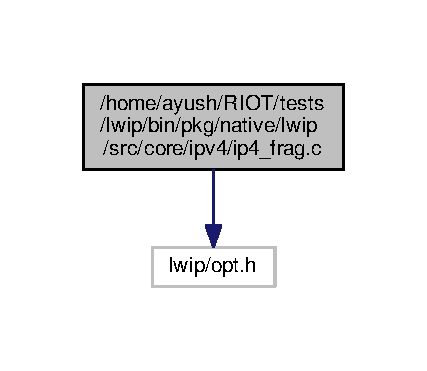
\includegraphics[width=205pt]{native_2lwip_2src_2core_2ipv4_2ip4__frag_8c__incl}
\end{center}
\end{figure}


\subsection{Detailed Description}
This is the I\+Pv4 packet segmentation and reassembly implementation. 